
\chapter{Static gestures recognition}\label{staticChapter}

As mentioned in Subsection~\ref{DynamicStaticText}, the gestures can be divided into two main groups: static gestures and dynamic gestures.
The static gestures can be understood as a position and orientation of fingers and a hand in a single moment. The dynamic gestures are defined as a movement of hands in time. 
The problem of static gesture recognition is a subject of this chapter. 
The proposed approach is presented, followed by the introduction to the evaluation scheme. 
In the last section, the performed experiments are described, which were used to examine the effectiveness of proposed approach.

\section{Proposed methods}

The static gesture recognition problem can be stated as a problem invariant to time.
That means that for each detected hand, it's position and orientation can be treated as a new data point, uncorrelated to previously shown gestures.
With this assumption, one can easily generate multiple samples from the sensors in short time, but it also gives an opportunity to look at the static gesture recognition problem as a problem of classification.

In literature, most of the approaches uses two-dimensional representation of gestures, which makes recognition problems relatively simple and therefore allows to use simple classification algorithms, e.g., k-NNs \cite{gestureRecognitionToolbox}. 
The three-dimensional representation of data is more complicated to model by the set of features and finally successfully label.
The 3D data yield by the sensor is represented in the sensor's coordinate system. 
Due to this fact, even a small change of the position or orientation of a hand with respect to the location of the sensor can negatively affect the gesture recognition system.
All of those distortions should not prevent the system from recognizing those gestures if they are similar.
To meet those requirement, it is needed to define what is the ``small'' change in orientation resulting in treating the static gestures as the same one.

\begin{figure}[htb]
\centering
 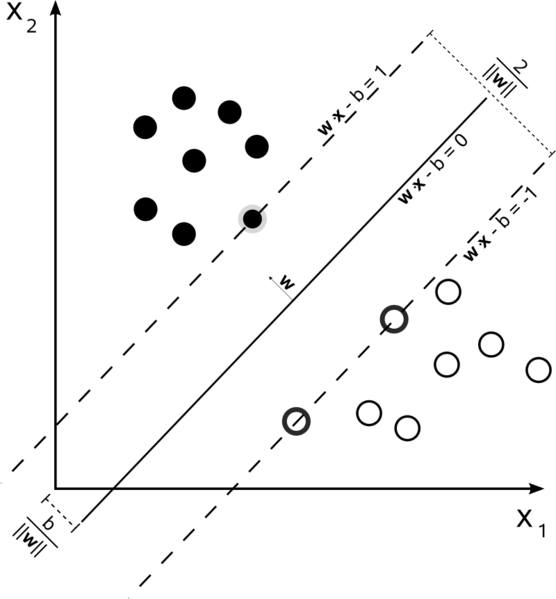
\includegraphics[width=0.6\columnwidth]{figures/SVM.png}
 \caption[]{SVM is a classification algorithm looking for the hyperplane that maximizes the margin between classes\footnotemark}
 \label{svmmargin}
\end{figure}

In application of the library presented in this thesis, it is assumed that the learning process can be done offline, while strict online requirements has to be met for the recognition part. 

To meet listed requirements, the Support Vector Machines (SVMs)\cite{Cortes:SVM} were used as a robust classification algorithm.
The SVMs were chosen as there exist a solid mathematical background supporting the simple idea of maximizing the margin between classes.
The SVMs are popular in the recent research trends and are commonly used in biology, robotics or IT for solving data classification problems.
Another advantage is the existence of the open-source library libSVM \cite{libSVM}, which contains an efficient implementation of the SVM in many programming languages.
In the original work, SVMs were designed to be able to classify between two classes, but the idea was expanded to utilize the one-vs-all classification allowing to differentiate between multiple classes.
This might be a drawback, as for $n$ classes, it is necessary to train $n$ SVMs, each to classify one class against all samples from the rest of the classes. 
The efficiency of SVMs depends on correctly choosing the kernel function used to map the separation problem into higher dimension with expectation to achieve a classification problem that can be separated.
There exists several kernel functions:
\begin{itemize}
\item linear: $K(x_i, x_j) = x_i^Tx_j$,
\item polynomial: $K(x_i, x_j) = (\gamma x_i^Tx_j + r)^d, \gamma > 0$,
\item radial basis function (RBF): $K(x_i, x_j) = exp(-\gamma ||x_i - x_j||^2), \gamma > 0$,
\item sigmoid: $K(x_i, x_j) = tanh(\gamma x_i^Tx_j+r)$,
\end{itemize}
where $\gamma$, $r$, and $d$ are kernel parameters. 
According to the authors of the library \cite{libSVM}, linear kernels perform the best, when used for linearly separable problems, while RBF kernels are the most versatile ones and are recommended for most of the applications.

\footnotetext{\url{http://en.wikipedia.org/wiki/File:Svm_max_sep_hyperplane_with_margin.png}}

The problem of classification assumes that each sample consists of set of features, which describe a sample and can be used to distinguish it from the other samples.
Additionally, each sample has a known or unknown label, which define the membership of the sample to the classification class. 
The samples with known labels can be used to train the classification system.
The trained classification system is used to predict the labels for the unlabelled samples.

In application of gesture recognition the classification is divided into two modes: the training part (offline) and the recognition part (online). 
The static gesture processing flow is presented in Fig.~\ref{staticsol}.
In the training part, the library is provided with the recorded, labelled samples of static gestures. 
From those samples, the sets of features are computed, which are used to train the classifier.
The recognition part assumes to have trained classifier. 
The recognition part is provided with samples of static gestures without labels. 
For each sample the sets of features are computed and then given as input to the trained classifier.
The classifier provides the information of the predicted gesture's class membership (label) for each input sample.

\begin{figure}[htb]
\centering
 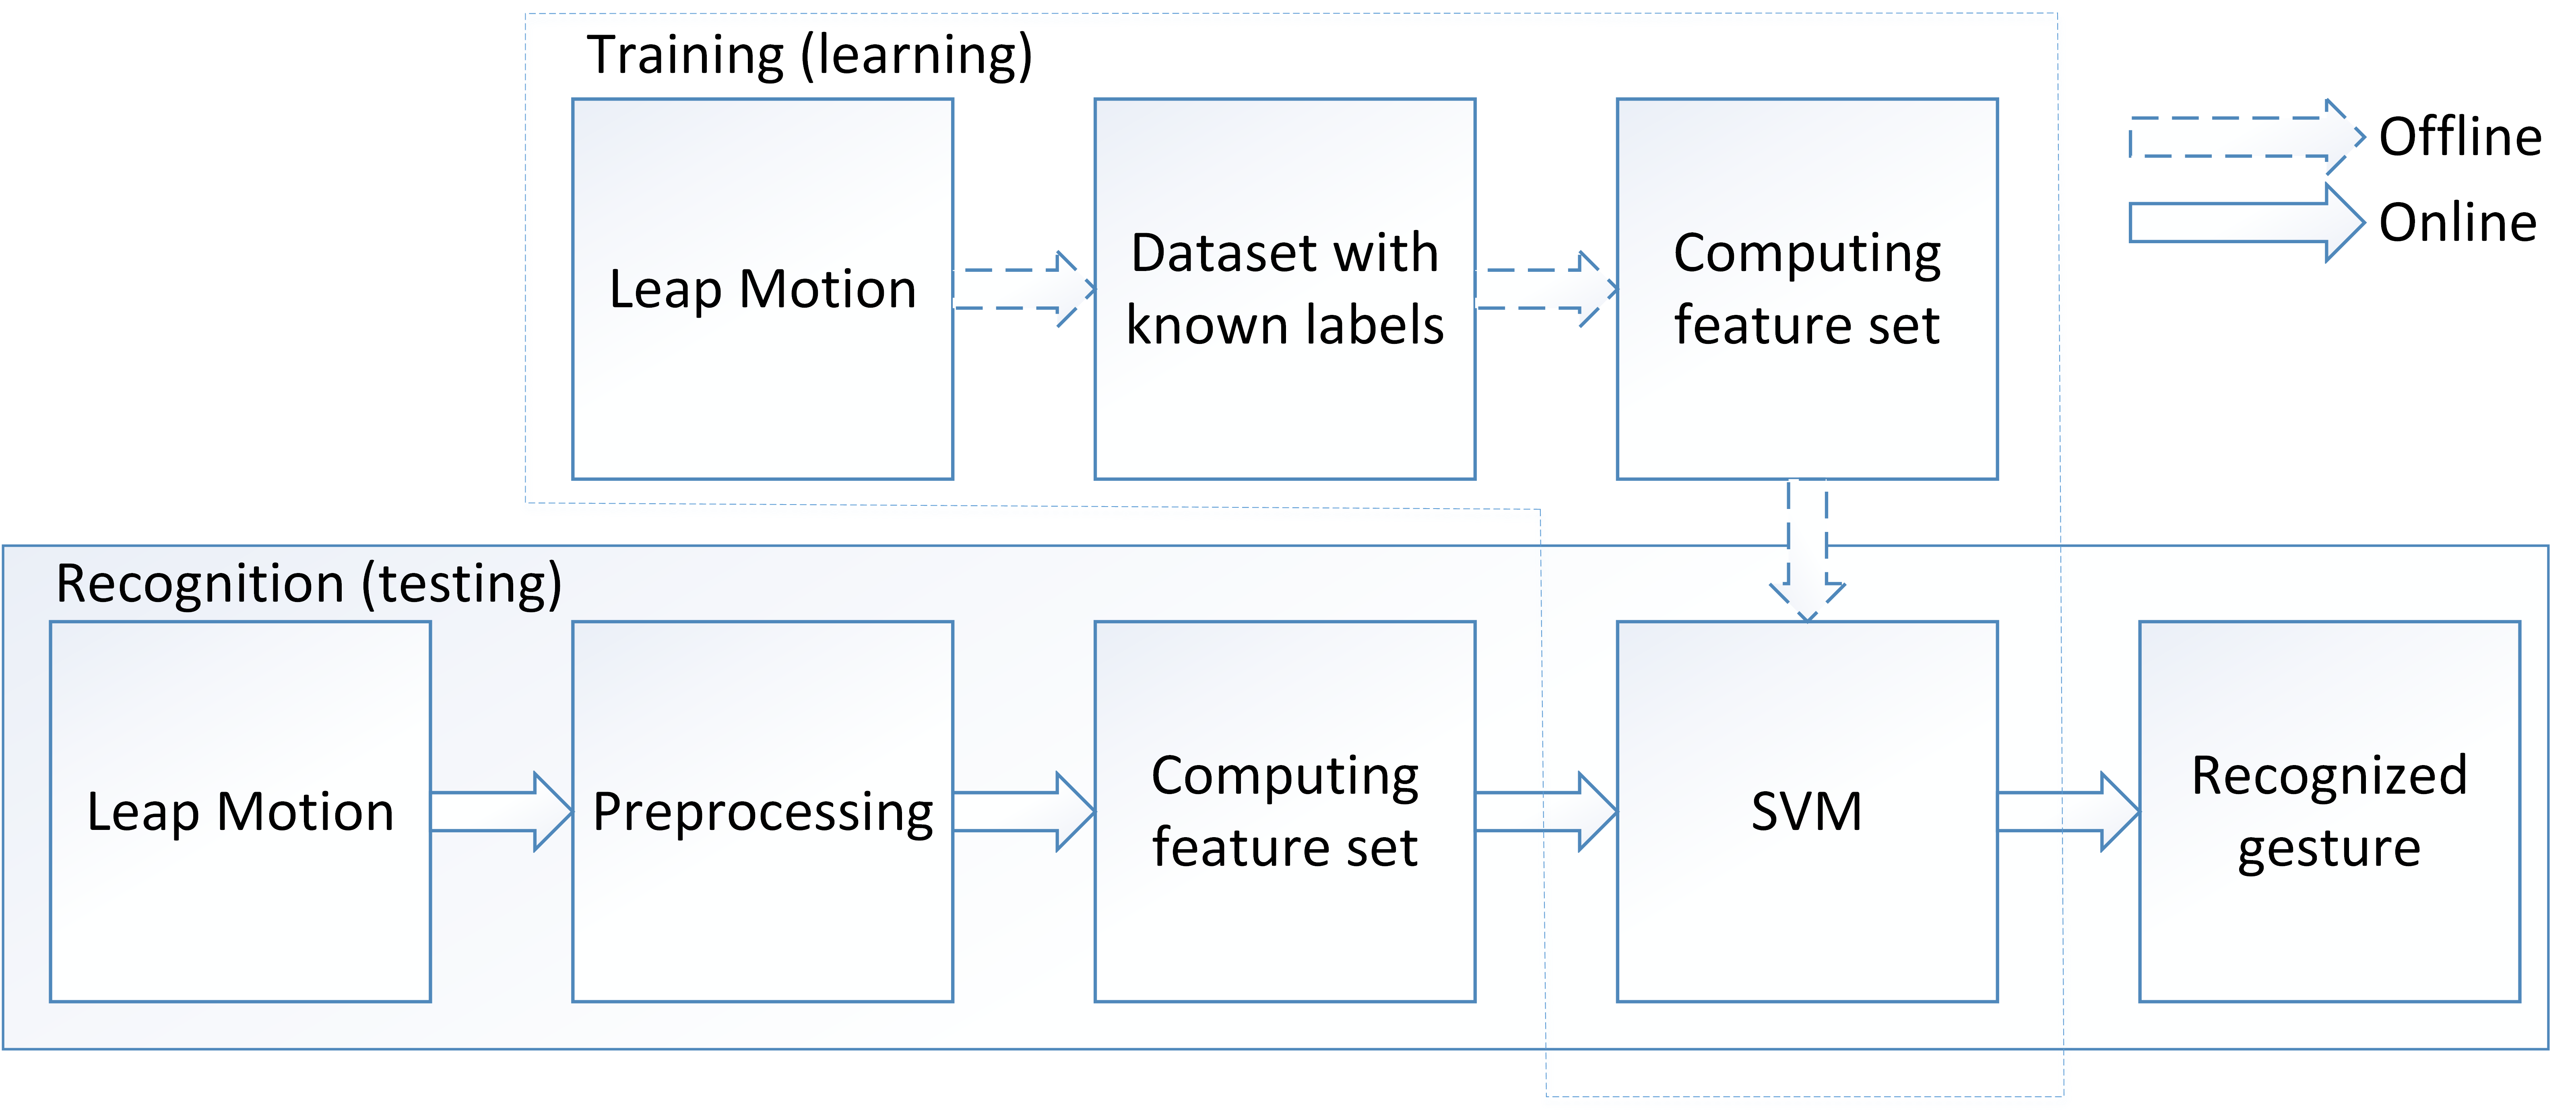
\includegraphics[width=1\columnwidth]{figures/StaticGestures.png}
 \caption[]{Proposed solution blocks for learning and recognition parts of static gestures recognition problem}
 \label{staticsol}
\end{figure}

While the presented approach can be treated as state-of-the-art approach it still cannot be used without defining proper feature sets for gesture recognition.
The naive solution would be to use the raw data from Leap Motion sensor as the feature set.
This solution was tested, but provided poor results as the raw data points are dependent on the position, orientation and scale of hand. 
Even a small movement in any direction resulted in decrease of classification accuracy.
The literature suggests to compute a set of features invariant to wanted transformations, which can allow to fully distinguish between different classes \cite{BishopML,libSVM}.
To achieve feature set with those properties, is has to been introduced taking into account the application.
Also, as the gesture recognition problem using the data similar to the data provided by the Leap Motion sensor has not been yet examined by the researches, seeking right feature set is a task of the thesis.
The task is approached in experimental Section~\ref{static:exp}.

\section{Evaluation Methodology}

\subsection{Assumptions}\label{staticAssumptions}
To provide a user with a library working in different conditions, it was assumed that a gesture is treated as the same one independently with respect to the translation, rotation and scale of the hand. 
This assumption means that the static gesture rotated by unknown angles, translated in the sensor coordinate system and also with different hand sizes should still be recognized as the same gesture.
Invariance to the rotation, translation and scale poses a great challenge to the recognition, but allows the future users of API to fully utilize the power of the library.
It is worth mentioning that, it does not reduce the possible applications of the library, as an assignment of a static gesture to an already defined class allows to find the transformation between the model of the class and the observed gesture.
This transformation can be used to examine the parameters of the instance of the model, e.g., rotation of the hand.

\subsection{Recorded Datasets}

To propose and test the quality of the features twelve static gestures were chosen:
\begin{enumerate}
\item the peace sign,
\item a fist,
\item full hand with space between each finger,
\item ``I love you'' sign from American Sign Language,
\item sign ``gun'' created by putting thumb and forefinger up, while holding the rest fingers in a fist,
\item all fingers in a fist with exception of thumb, which is up,
\item the sign X made with the forefingers of both hands,
\item the sing ``Time'' used e.g. by coaches in basketball games.
\item sign simulating rotating a knob by two fingers,
\item sign simulating rotating a knob by five fingers.
\end{enumerate} 

\begin{figure}[htb]
\centering
 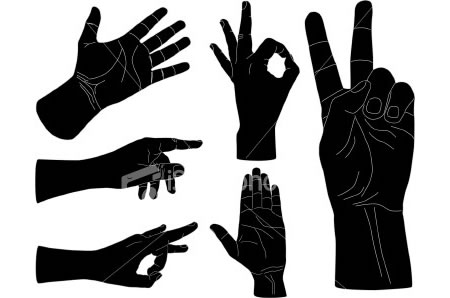
\includegraphics[width=1.0\columnwidth]{figures/static_gestures.png}
 \caption{Recorded static gestures used for evaulation}
 \label{staticgesturesdata}
\end{figure}
The gestures are also presented in Fig.~\ref{staticgesturesdata}.

The sample data of each gestures were recorded using the continuous mode of recording, while moving the hands in different directions and changing the orientation of the hands.
The hands were moved and rotated as each repeated static gesture is always a little bit different from the previously recorded samples.
In total, for each of the proposed classes, each author of this thesis recorded approximately 1000 samples.

Having samples with known labels, the whole dataset was separated into training and testing sets in relation $2:1$. 
For the training, the k-fold cross-validation (CV) scheme was used, which searches for optimal $C$ and $\gamma$ parameters of SVM.
This method is used to find the optimal parameters of the classification system, while estimating the performance is done on the testing data not used in the training part. 
In a standard version of the CV, the gathered data is divided into two sets: one containing $k-1$ parts of the data and the other $1$ part of the data. 
The first is used to train the classification system, while the rest of the gathered data is used to estimate how well the system is learnt.
In the next iteration, the CV parts are shuffled by still having the ratio of training and validation sets.
After the training, the final performance is estimated by calculating the percent of correctly recognized labels to the total size of the testing set.


\section{Experiments}
\label{static:exp}

\subsection{Evaluation of feature sets}

The goal of the first experiments was to find the proper set of features. Several feature sets were proposed and tested. The first vector of features consisted of:
\begin{itemize}
\item number of fingers in a frame,
\item euclidean distances between consecutive finger's tips,
\item absolute angles between consecutive fingers.
\end{itemize} 

This feature set did not take into account the relative position of fingers to the hand.
The second feature set is the first feature set extended by the distances between consecutive finger tips and the position of the hand's palm.
The third feature set contains features from the second feature set extended by the five angles between fingers and normal of hand's palm.
The firstly tested set of all static gestures contained gestures, which were undistinguishable for the Leap Motion, because they did not take into account the way, the Leap Motion works. 
For gestures like fist, the recorded data contained almost no information how to classify those gestures.
That's why the experiments were repeated on the five gestures, which could be easily distinguish using the data provided by Leap Motion. 
For this experiment the gestures peace, hand, ''I love you'', fist with thump up and rotating knob by 5 fingers were chosen.
The results achieved by those methods are presented in Table~\ref{staticfeat}.

\begin{table}[htp!]
	\label{staticfeat}
	\caption{Results obtained by proposed feature sets using the libSVM library}
    \begin{tabular}{ccccc}
    \hline
    ~                                                   & $5$ gestures, CV & $5$ gestures, test set & $10$ gestures, CV  & $10$ gestures, test set \\ \hline
    feature set $1$                     & $87.1\%$ & $87.9\%$ & $70.0\%$ & $68.4\%$   \\ \hline
    feature set $2$                     & $87.1\%$ & $87.9\%$ & $70.0\%$ & $68.4\%$          \\ \hline
    feature set $3$                     & $87.1\%$ & $87.9\%$ & $70.0\%$ & $68.4\%$           \\ \hline
    feature set $4$                     & $81.2\%$ & $81.0\%$ & $68.4\%$ & $68.6\%$          \\ \hline
    feature set $5$                     & $86.5\%$ & $85.1\%$ & $77.1\%$ & $77.5\%$          \\ \hline
    feature set $6$                     & $92.8\%$ & $93.1\%$ & $80.5\%$ & $81.2\%$           \\ \hline
    \end{tabular}
\end{table}

For the problem of recognition of five gestures, three first feature sets resulted in over $87\%$ recognition rate on testing sets.
The same tests for the problem of recognition of $10$ gestures resulted in lower recognition rates.
For feature sets 1--3 the recognition rate was below $70\%$, which could be unsatisfying from the perspective of the purpose of the application.
The low recognition rate was analysed.  
The analysis revealed that the fingers are numbered by Leap Motion accordingly to the position in Z axis of the tip of the finger.
This means that when finger's tips are approximately on the same position in Z axis, the numbering can change rapidly and proposed features are compared between different fingers.
To achieve features that would be invariant to the numbering of the fingers, the feature set was slightly modified.
Instead of containing the absolute angles and distances between consecutive fingers, it was proposed to contain the five greatest values of angles and five greatest values of distances between all combinations of finger pairings.
The same sorting approach was used for the angles and distances between fingers and hand's palm.
The feature sets $1$, $2$, $3$ with sorting scheme were respectively called feature sets $4$, $5$, $6$.
Again, the same dataset with $5$ and $10$ gestures was used to evaluate those methods. 
The results are presented in Table~\ref{staticfeat}.
This approach was tested on the same training set and allowed to increase the recognition rate.
The best results in both tasks were achieved in case of feature sets $6$.
The simple alleviation of finger numbering problem allowed to top the previous results with recognition rates $93.096\%$ for $5$ gesture problem and $81.235\%$ for $10$ gestures problem. 

\begin{table}[htp!]
\begin{center}
	\label{staticfeatlin}
	\caption{Results obtained by proposed feature sets using the libLinear library}
    \begin{tabular}{ccccc}
    \hline
    ~                                                   & $5$ gestures, CV & $5$ gestures, test set & $10$ gestures, CV  & $10$ gestures, test set \\ \hline
    feature set $1$                     & $78.3\%$ & $78.3\%$  & $50.6\%$ & $50.6\%$ \\ \hline
    feature set $2$                     & $78.3\%$ & $78.3\%$  & $50.6\%$ & $50.6\%$ \\ \hline
    feature set $3$                     & $78.3\%$ & $78.3\%$  & $50.6\%$ & $50.6\%$ \\ \hline
    feature set $4$                     & $78.2\%$ & $78.2\%$  & $50.7\%$ & $50.6\%$ \\ \hline
    feature set $5$                     & $79.5\%$ & $79.5\%$  & $55.3\%$ & $55.3\%$ \\ \hline
    feature set $6$                     & $88.1\%$ & $88.1\%$  & $64.7\%$ & $64.8\%$ \\ \hline
    \end{tabular}
    \end{center}
\end{table}

While using more data and longer feature sets usually allows to achieve better results, it is worth to notice the increased learning time. 
In case of $5000$ training samples the typical training process of radial SVM took approximately $12$ hours on a desktop PC with Intel Core i7 and 6 GB of RAM. 
This computing time can be unacceptable by the users of the library. 
This is why the tests with another SVM library, libLinear~\cite{libLinear} were performed. 
The libLinear's implementation of SVM utilizes linear kernels and is dedicated for large data training sets with multiple number of features. 
This library reduced the training time to about $5$ seconds.
Again, the same tests as for the libSVM were performed to compare both approaches.
All achieved results are presented in Table~\ref{staticfeatlin}.
For the 5 gestures case, the libLinear achieved $88.1\%$ on the testing set while using feature set 6 compared to $93.1\%$ achieved by libSVM in the same condition.
In this case, the libLinear might be good choice as the recognition rate is lower only by about $5\%$.
For 10 gestures case, libLinear achieved $64.830\%$ compared to $81.235\%$ of LibSVM, which is a significantly lower recognition rate.
It's up to user to decide which library to use, but in most recognition applications, the library can be learnt offline and only used online.
That is why, the authors of this thesis recommend the SVM with RBF kernels for static gesture recognition task.

From the results obtained by the libSVM and libLinear on different feature sets, the feature set $6$ was chosen as the one yielding the best results and used in further analysis.

\begin{figure}[htb]
\centering
 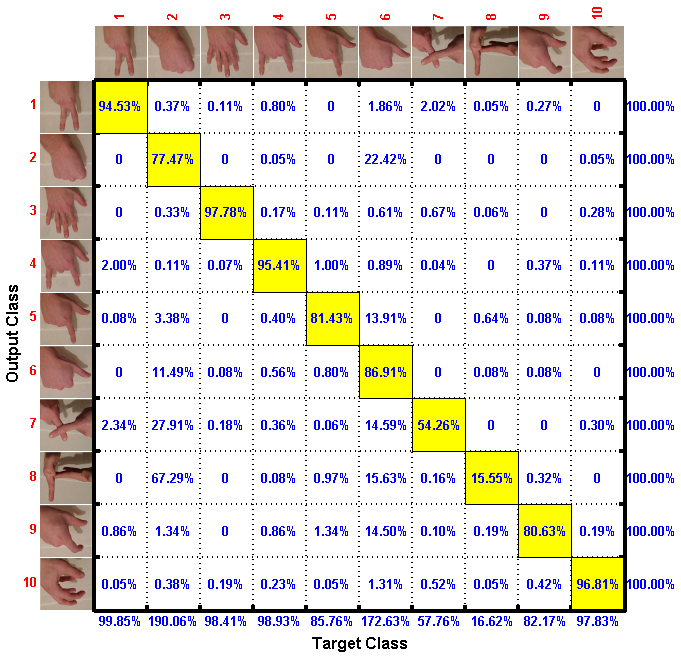
\includegraphics[width=0.8\columnwidth]{figures/staticClassesRecognitionRates.png}
 \caption{Recognition rates of classes for the feature set $6$}
 \label{staticClassesRecognitionRates}
\end{figure}

For the problem of recognition of $10$ gestures were performed an additional experiment on the test set, which presents the recognition rates achieved for each class. As a result, can be checked, for which gesturesselected feature set was the best, and for which was wrong. The fig.~\ref{staticClassesRecognitionRates} shows the results of the experiment in the form of confusion matrix. Gestures of two hands fared the worst. The reason for such low recognition rate errors can be reading error from the device, which performs poorly with overlapping objects. For gesture ``Time'' additional problems which may affect the reading of data, can be hand position perpendicular to the Leap Motion and join the finger tips of one palm to the other. Can be also noticed that the fist is often confused with exposed thumb gesture (no. $6$).

\subsection{Preprocessing}

Another factor, that might have an influence on the results is the preprocessing part, which should allow to partially remove noise from the data and thus increase the recognition rates. 
The preprocessing has been presented in Section~\ref{preprocessingSection}.
The preprocessing operates in the window of hands poses recorded over time, which size can be modified. 
The typical library usage allowed to gather data with $60Hz$, while it is assumed that the recognition can be performed with a lower framerate. The difference can be efficiently used by defining the appropriate preprocessing window.
For this reason, the experiments with no preprocessing and preprocessing with width size equal to $5$, $10$, $15$, $20$, $30$ were performed and the influence on the recognition rate was examined.
The results are presented in Table~\ref{staticpre}.
The achieved results confirm the need and importance of proper data preparation in task of data classification.
For gesture recognition task containing $5$ gesture poses, preprocessing allowed to increase the recognition rate from $93.1\%$ to over $99\%$ for window sizes equal or wider than $15$. 
In task of recognition 10 gestures, the preprocessing allowed to increase recognition rate from $81.2\%$ to over $84\%$ for windows sizes equal or wider than $10$.
From those results, the preprocessing width of $10$ was chosen as the one allowing to significantly improve recognition rate in almost any possible application of the library.
The preprocessing of width $10$ was used for all further experiments if not stated otherwise.

\begin{table}[htp!]
\begin{center}
	\label{staticpre}
	\caption{The recognition rate achieved with feature set $6$ and different sizes of preprocessing window}
    \begin{tabular}{ccccc}
    \hline
    preprocessing                                                   & $5$ gestures, CV & $5$ gestures, test set & $10$ gestures, CV  & $10$ gestures, test set \\ \hline
    off                     & $92.8\%$ & $93.1\%$  & $80.5\%$ & $81.2\%$ \\ \hline
    width = $2$               & $95.6\%$ & $96.5\%$  & $82.7\%$ & $83.2\%$ \\ \hline
    width = $5$               & $95.9\%$ & $96.7\%$  & $83.1\%$ & $83.6\%$ \\ \hline
    width = $10$              & $98.8\%$ & $99.0\%$  & $83.6\%$ & $84.1\%$ \\ \hline
    width = $15$              & $99.0\%$ & $99.2\%$  & $84.1\%$ & $84.5\%$ \\ \hline
    width = $20$              & $99.1\%$ & $99.2\%$  & $84.3\%$ & $84.8\%$ \\ \hline
    width = $30$              & $99.2\%$ & $99.4\%$  & $84.8\%$ & $85.3\%$ \\ \hline
    \end{tabular}
    \end{center}
\end{table}

\subsection{Postprocessing}


All of already presented experiments, treated the classification results of consecutive hand poses as time-independent and not correlated with each other.
In real applications, it can be safely assumed that the consecutively detected hands are similar to each other and probably define the same gesture.
The remaining question to be answered was the impact of combining the consecutive recognition results for the total recognition percentage.
It is important to use not only the class labels for the tested dataset, but the whole information provided by SVM containing the measure of classification rate to all possible classes.
This data can be combined to measure the membership rate for each class in a window of chosen width.
Then the predicted class is the class with maximal measure.
Formally, when there is a need to classify between $k$ classes, the result for $i$-th data in dataset can be represented as:
\begin {equation}
l(i) = [l_{i1}, l_{i2}, ..., l_{ik}],
\end{equation}
where $l_{ik}$ is the probability measure of $i$-th data belonging to the $k$-th class.
Using a window of width $w$, the new estimate of classes l' can be computed using the equation:
\begin{equation}
l'(i,w) = F( l(i-w), l(i+1-w), ..., l(i) ),
\end{equation}
where F represents the aggregation function with $w$ vector arguments, e.g., the sum of elements of each input vector.
The recognized label is the number of the vector component with the highest value:
\begin{equation}
\mathrm{label} = \argmax_{k}{\{r(i,w)_k\}}.
\end{equation}


\begin{figure}[htbp!]
\centering
 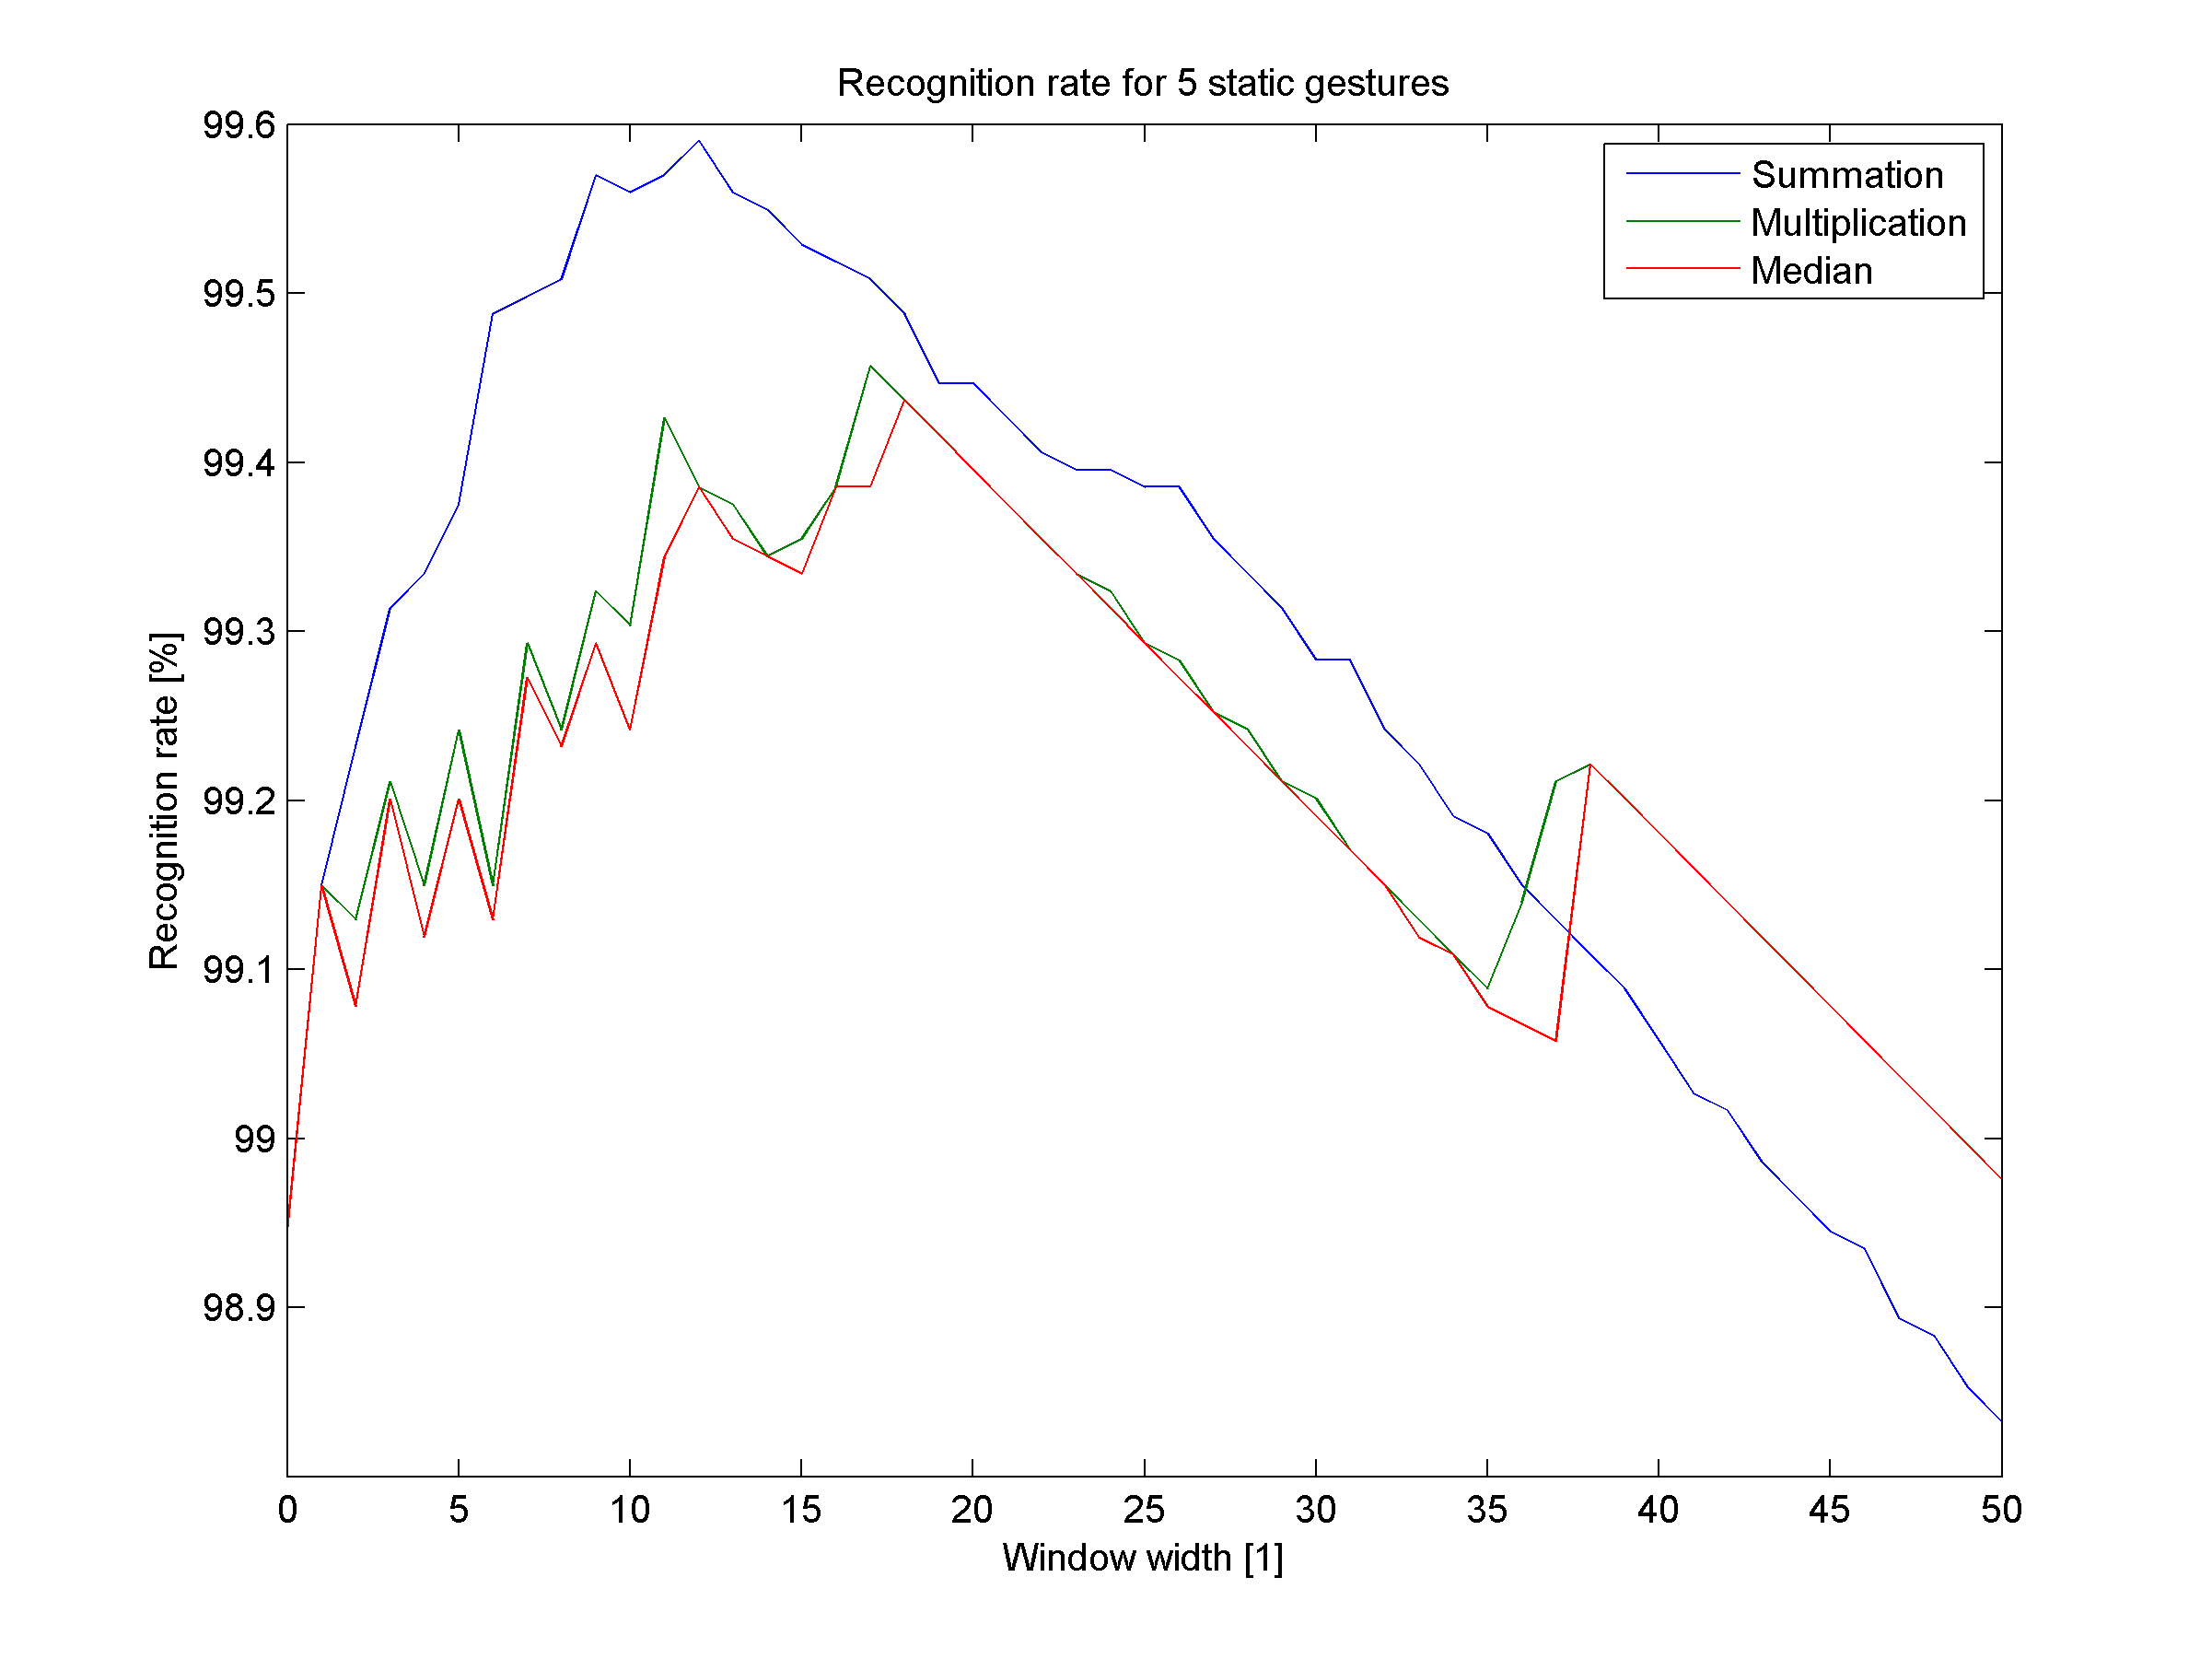
\includegraphics[width=0.7\textwidth]{figures/Mul5.png}
\centering 
 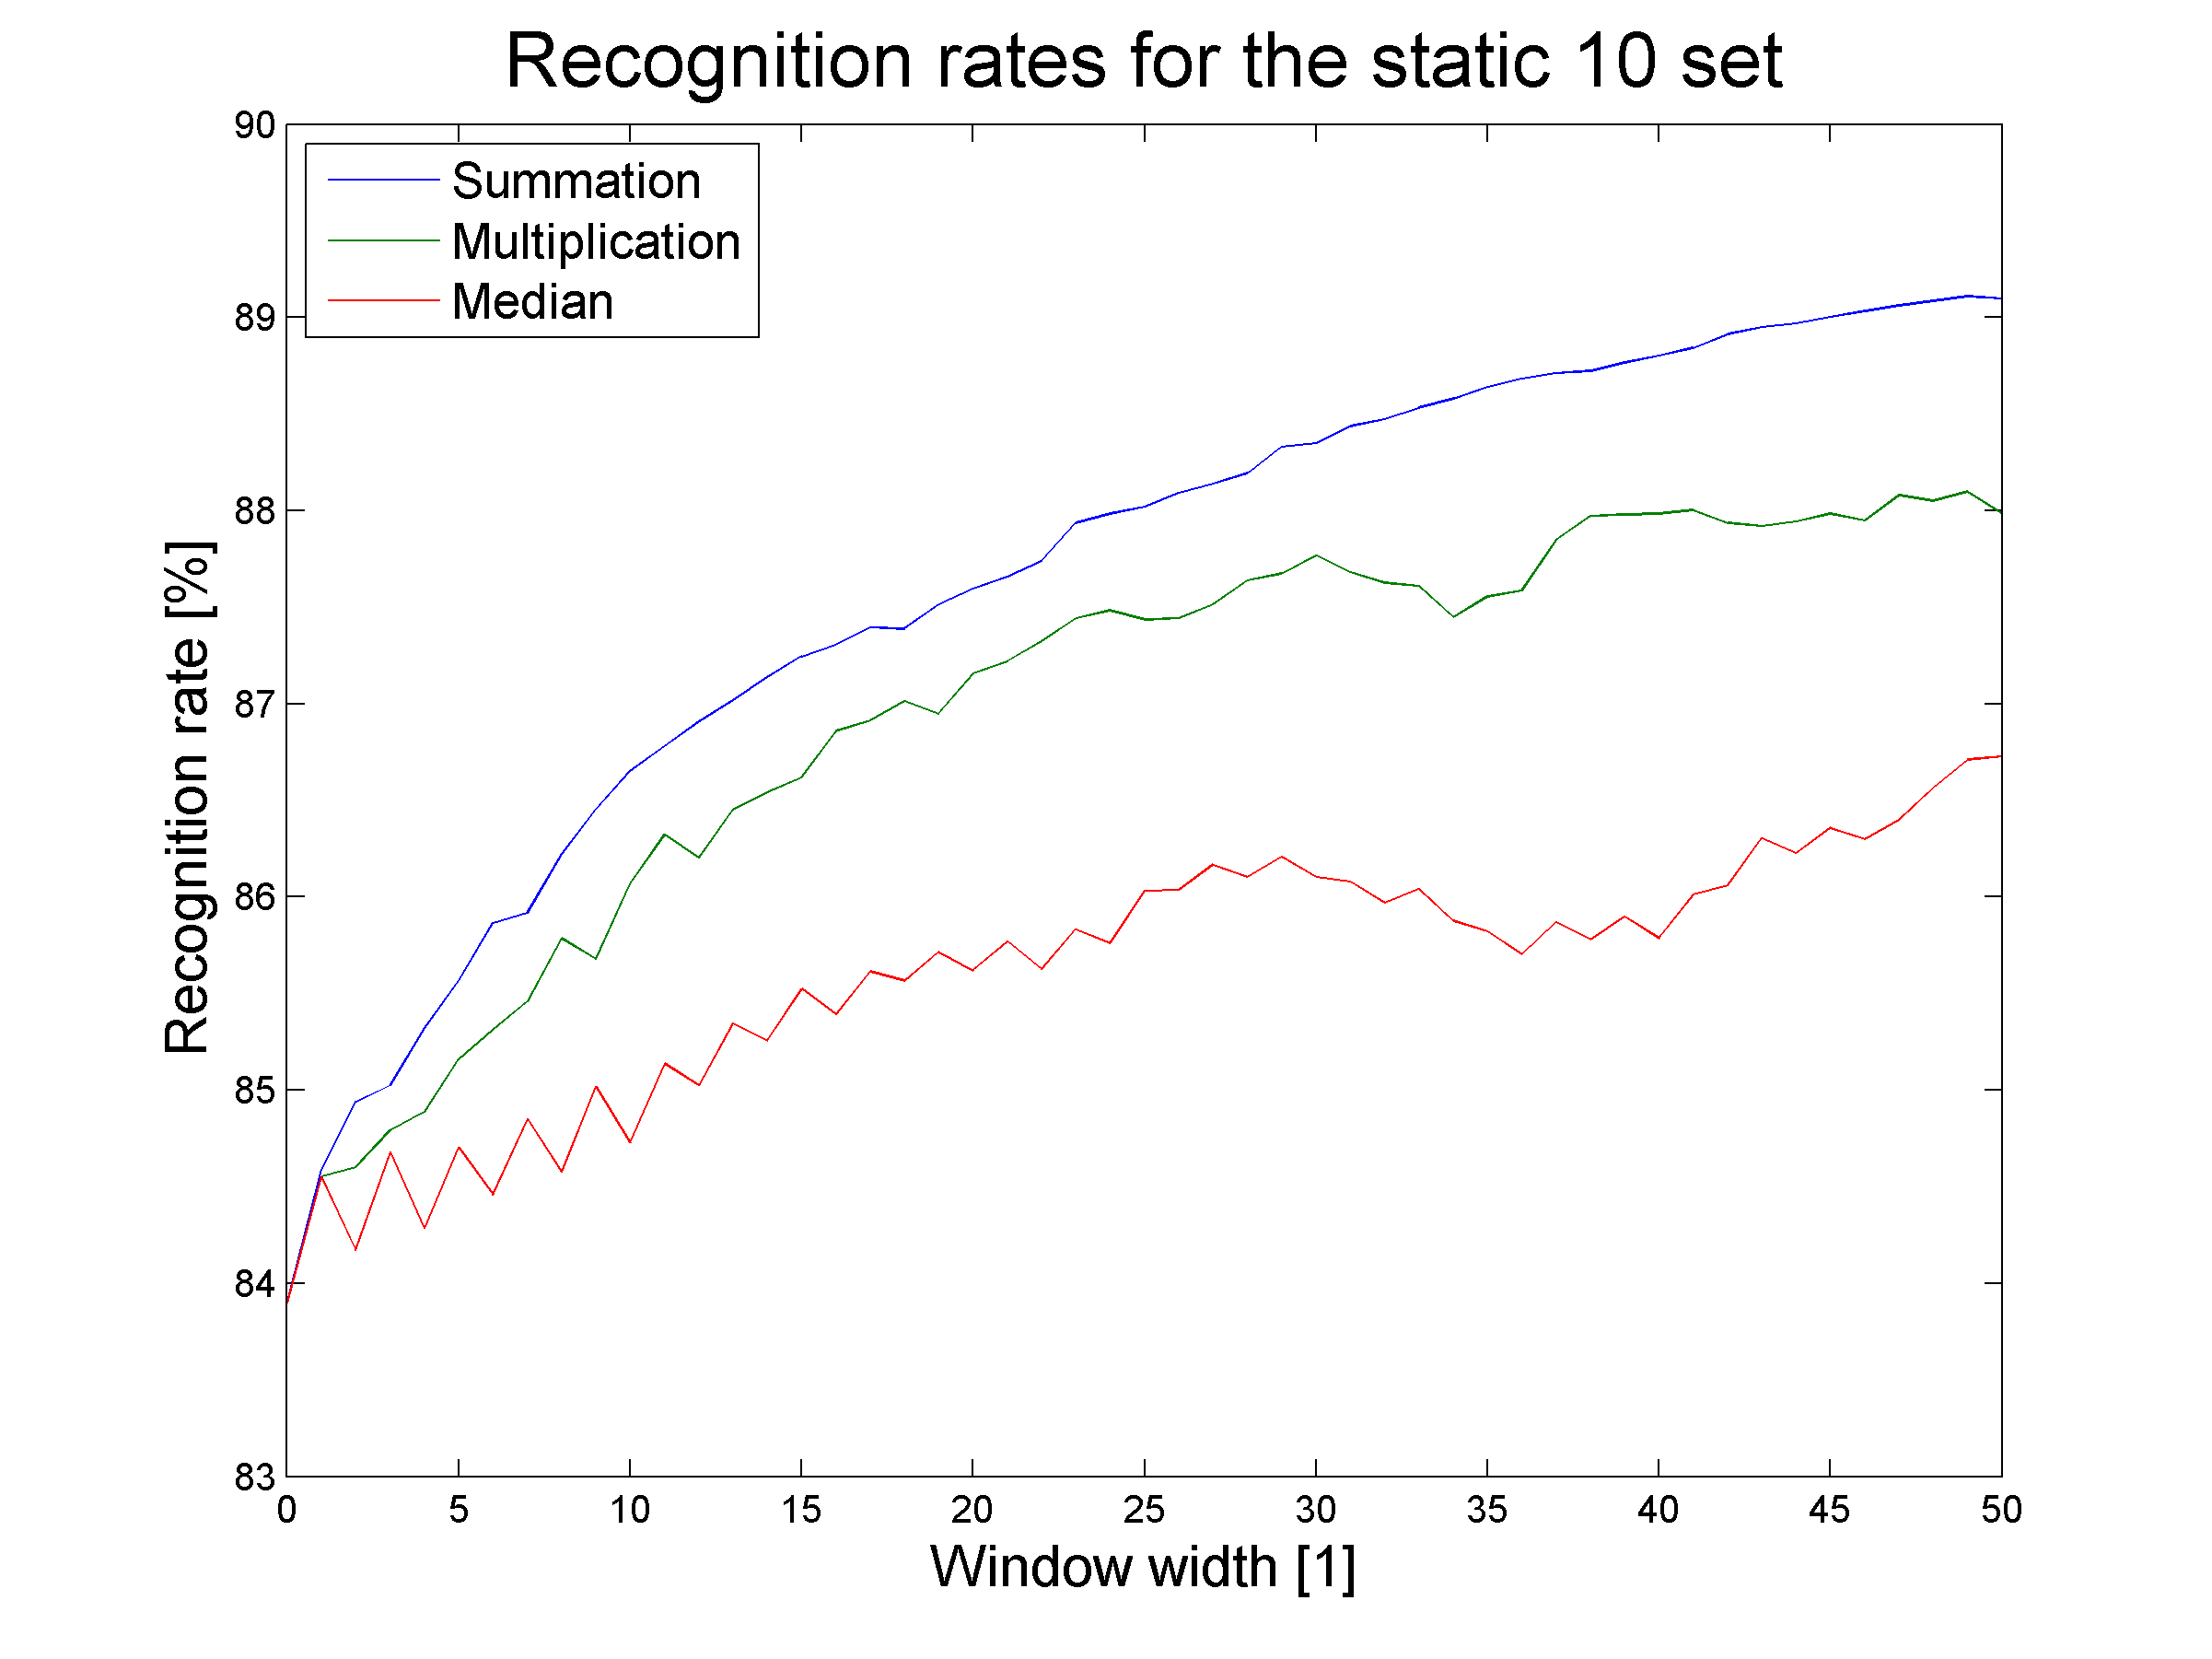
\includegraphics[width=0.7\textwidth]{figures/Mul10.png}
 \caption{Evaluation of different aggregation operators for result combining in case of different window sizes}
 \label{staticoper}
\end{figure}

 

The first approach to defining the sum operator is the operator of simple adding the elements of vectors $l$.
The second proposition is to multiple the corresponding elements of vectors $l$. 
The third approach utilizes the idea of calculating the median elements of vectors $l$.
The three approaches were compared using feature set 6 with preprocessing width equal to 10 for 5 and 10 gestures already used in previous experiments.
Simultaneously, the test were performed for different widths of window and are presented in Fig.~\ref{staticoper}.
For almost all possible widths, the summation operator demonstrated the best recognition rate.
For 5 static gestures, the summation with width equal to 10 allowed to achieve the recognition rate over $99.5$\% gaining over $0.5\%$ when compared to solution without postprocessing.
Interestingly, windows wider than 12 resulted in lower recognition rate than the result obtained by the window width equal to 10.
For 10 static gesture recognition problem, a window of size 50 allowed to improve the recognition rate by over $5\%$ to the value over $89$\%.
In this case, wider window resulted in better results. 
Similarly to the preprocessing window size, also in postprocessing too wide window results in delayed recognition rate of a shown gesture.
Also, too wide window may not lead to better results.
Therefore, the postprocessing window size of 10--15 is recommended by the authors of this thesis.


Using summation as the aggregation operator treats the currently achieved result and the results from the previous as equally affecting the current recognition. 
Especially for wider windows, it can be assumed that the current measurement is more important than the measurement from the distant past.
That is why, the idea of weighted sum was introduced.
The chosen weights should have the highest weight for the current measurement and smaller values for results that were achieved earlier in time.

\begin{figure}[htbp!]
\centering
 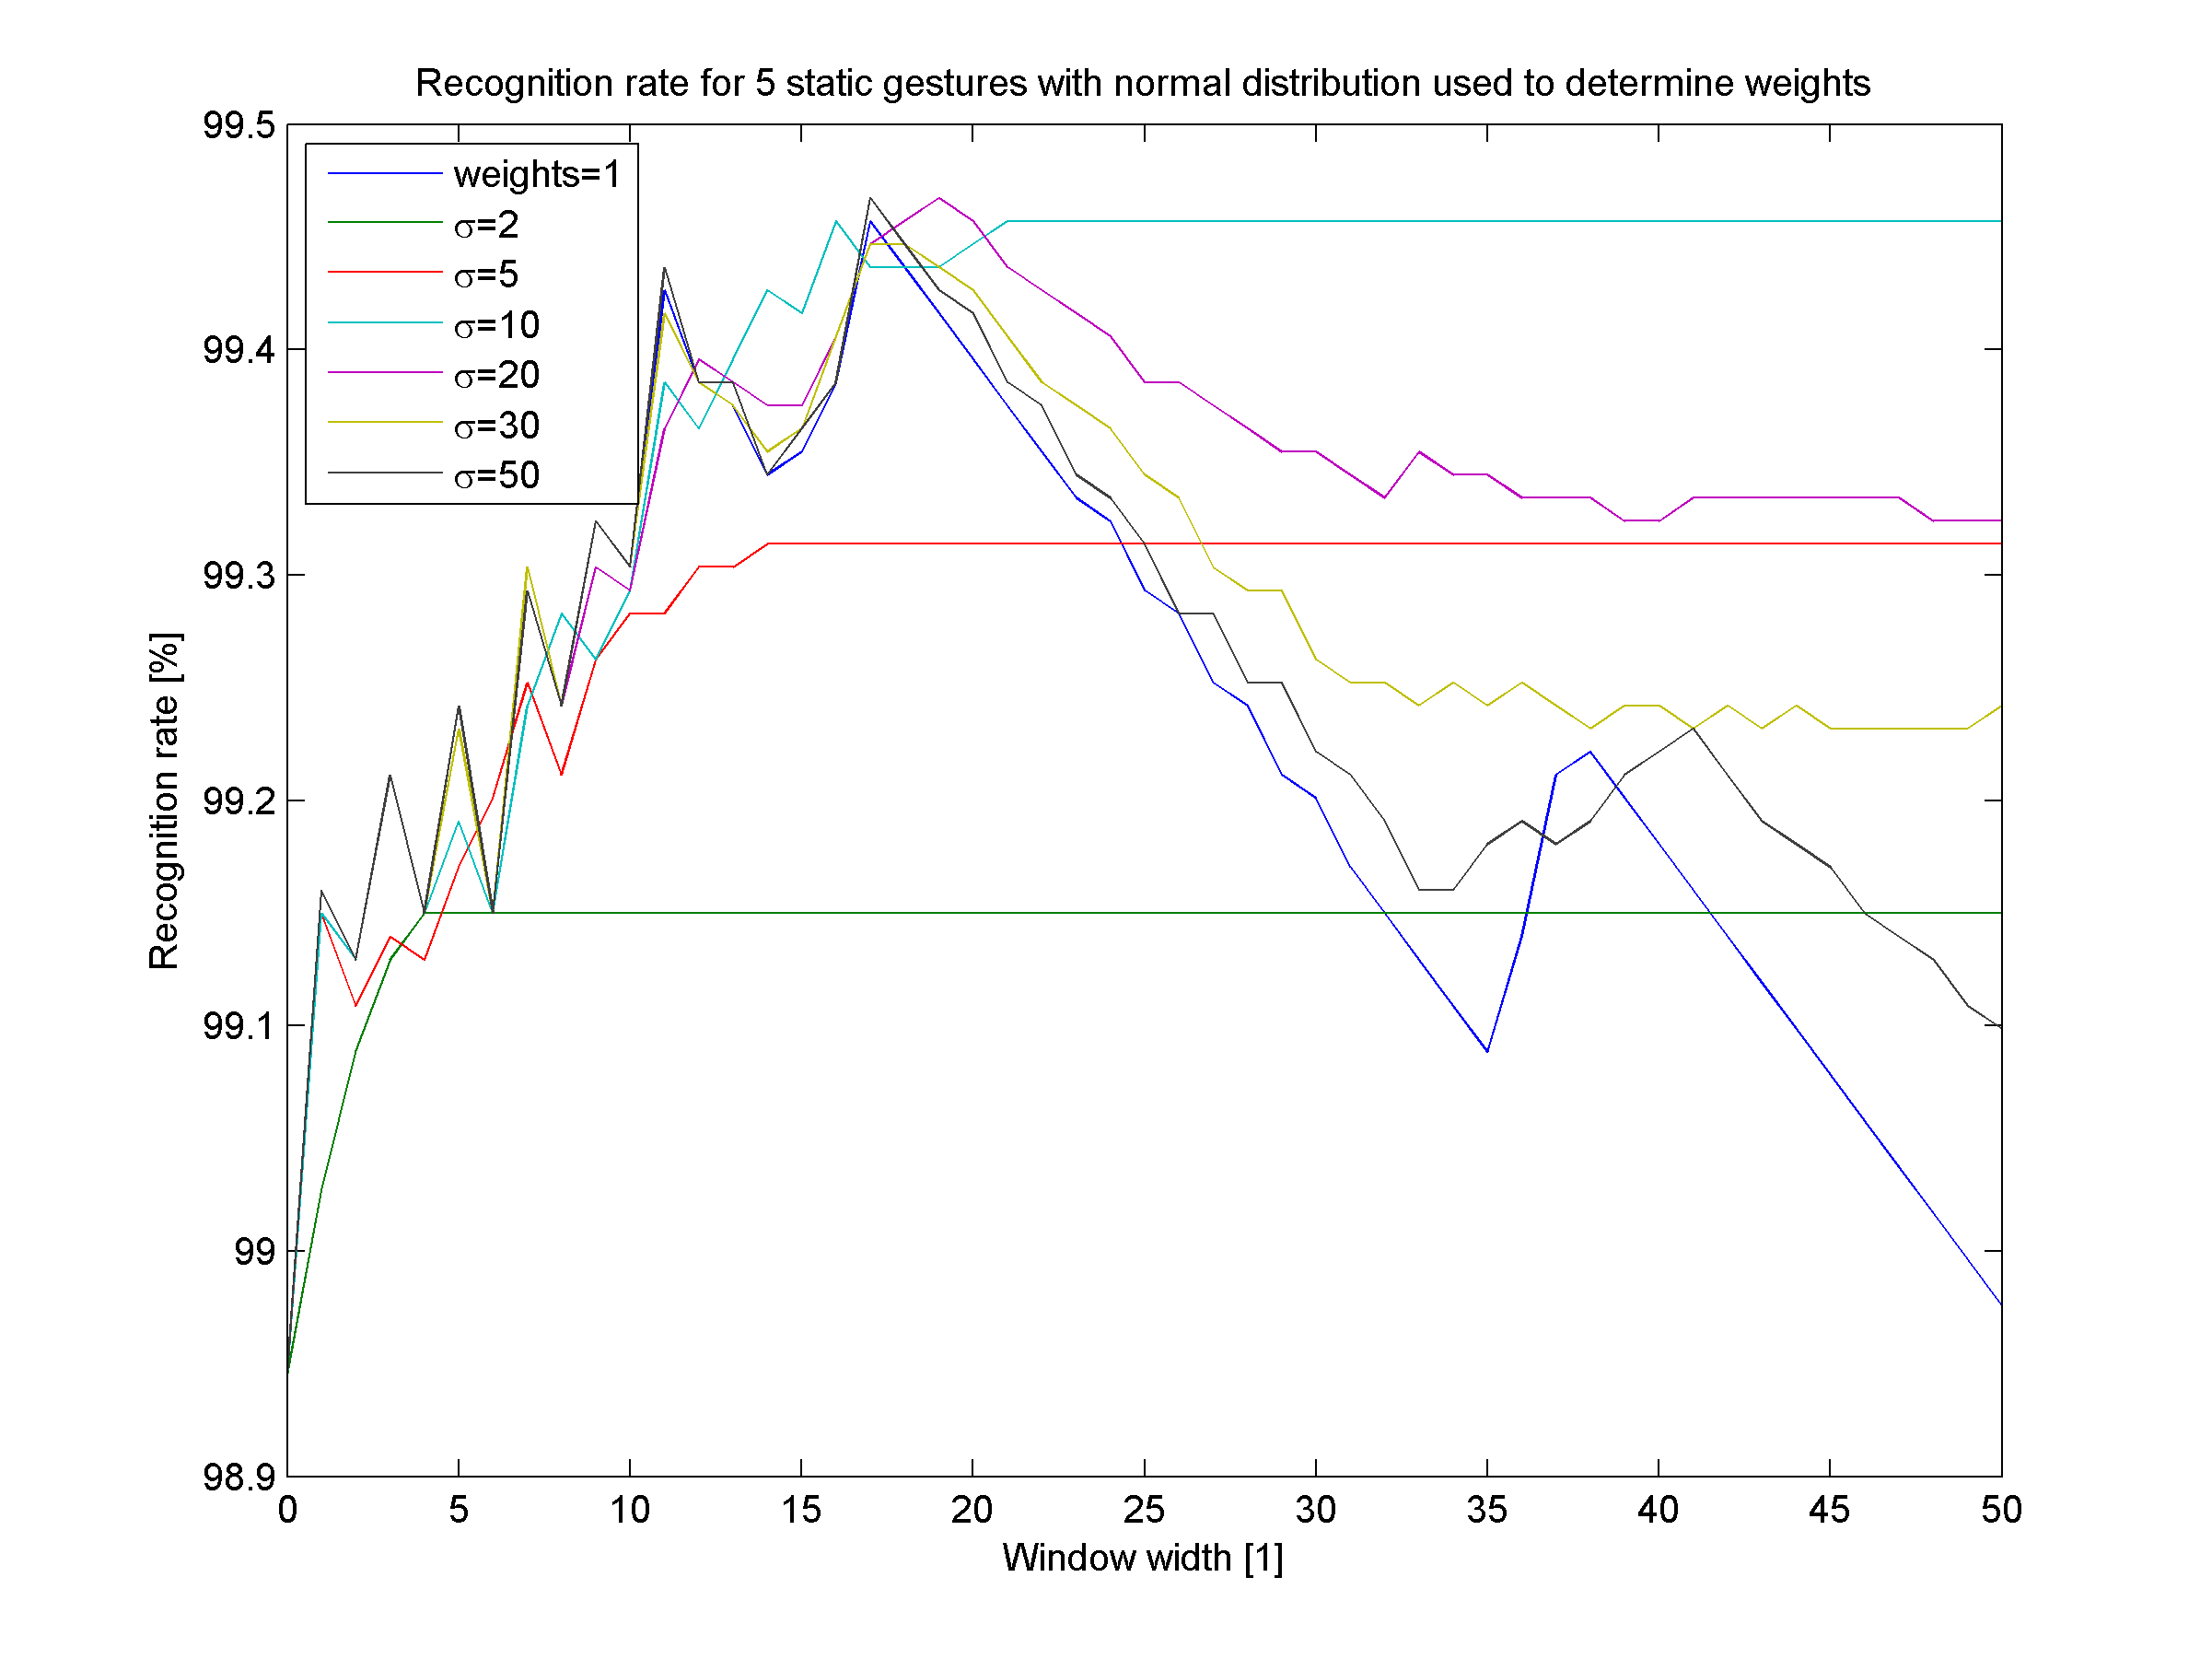
\includegraphics[width=0.7\textwidth]{figures/gaussSum5.png}
\centering
 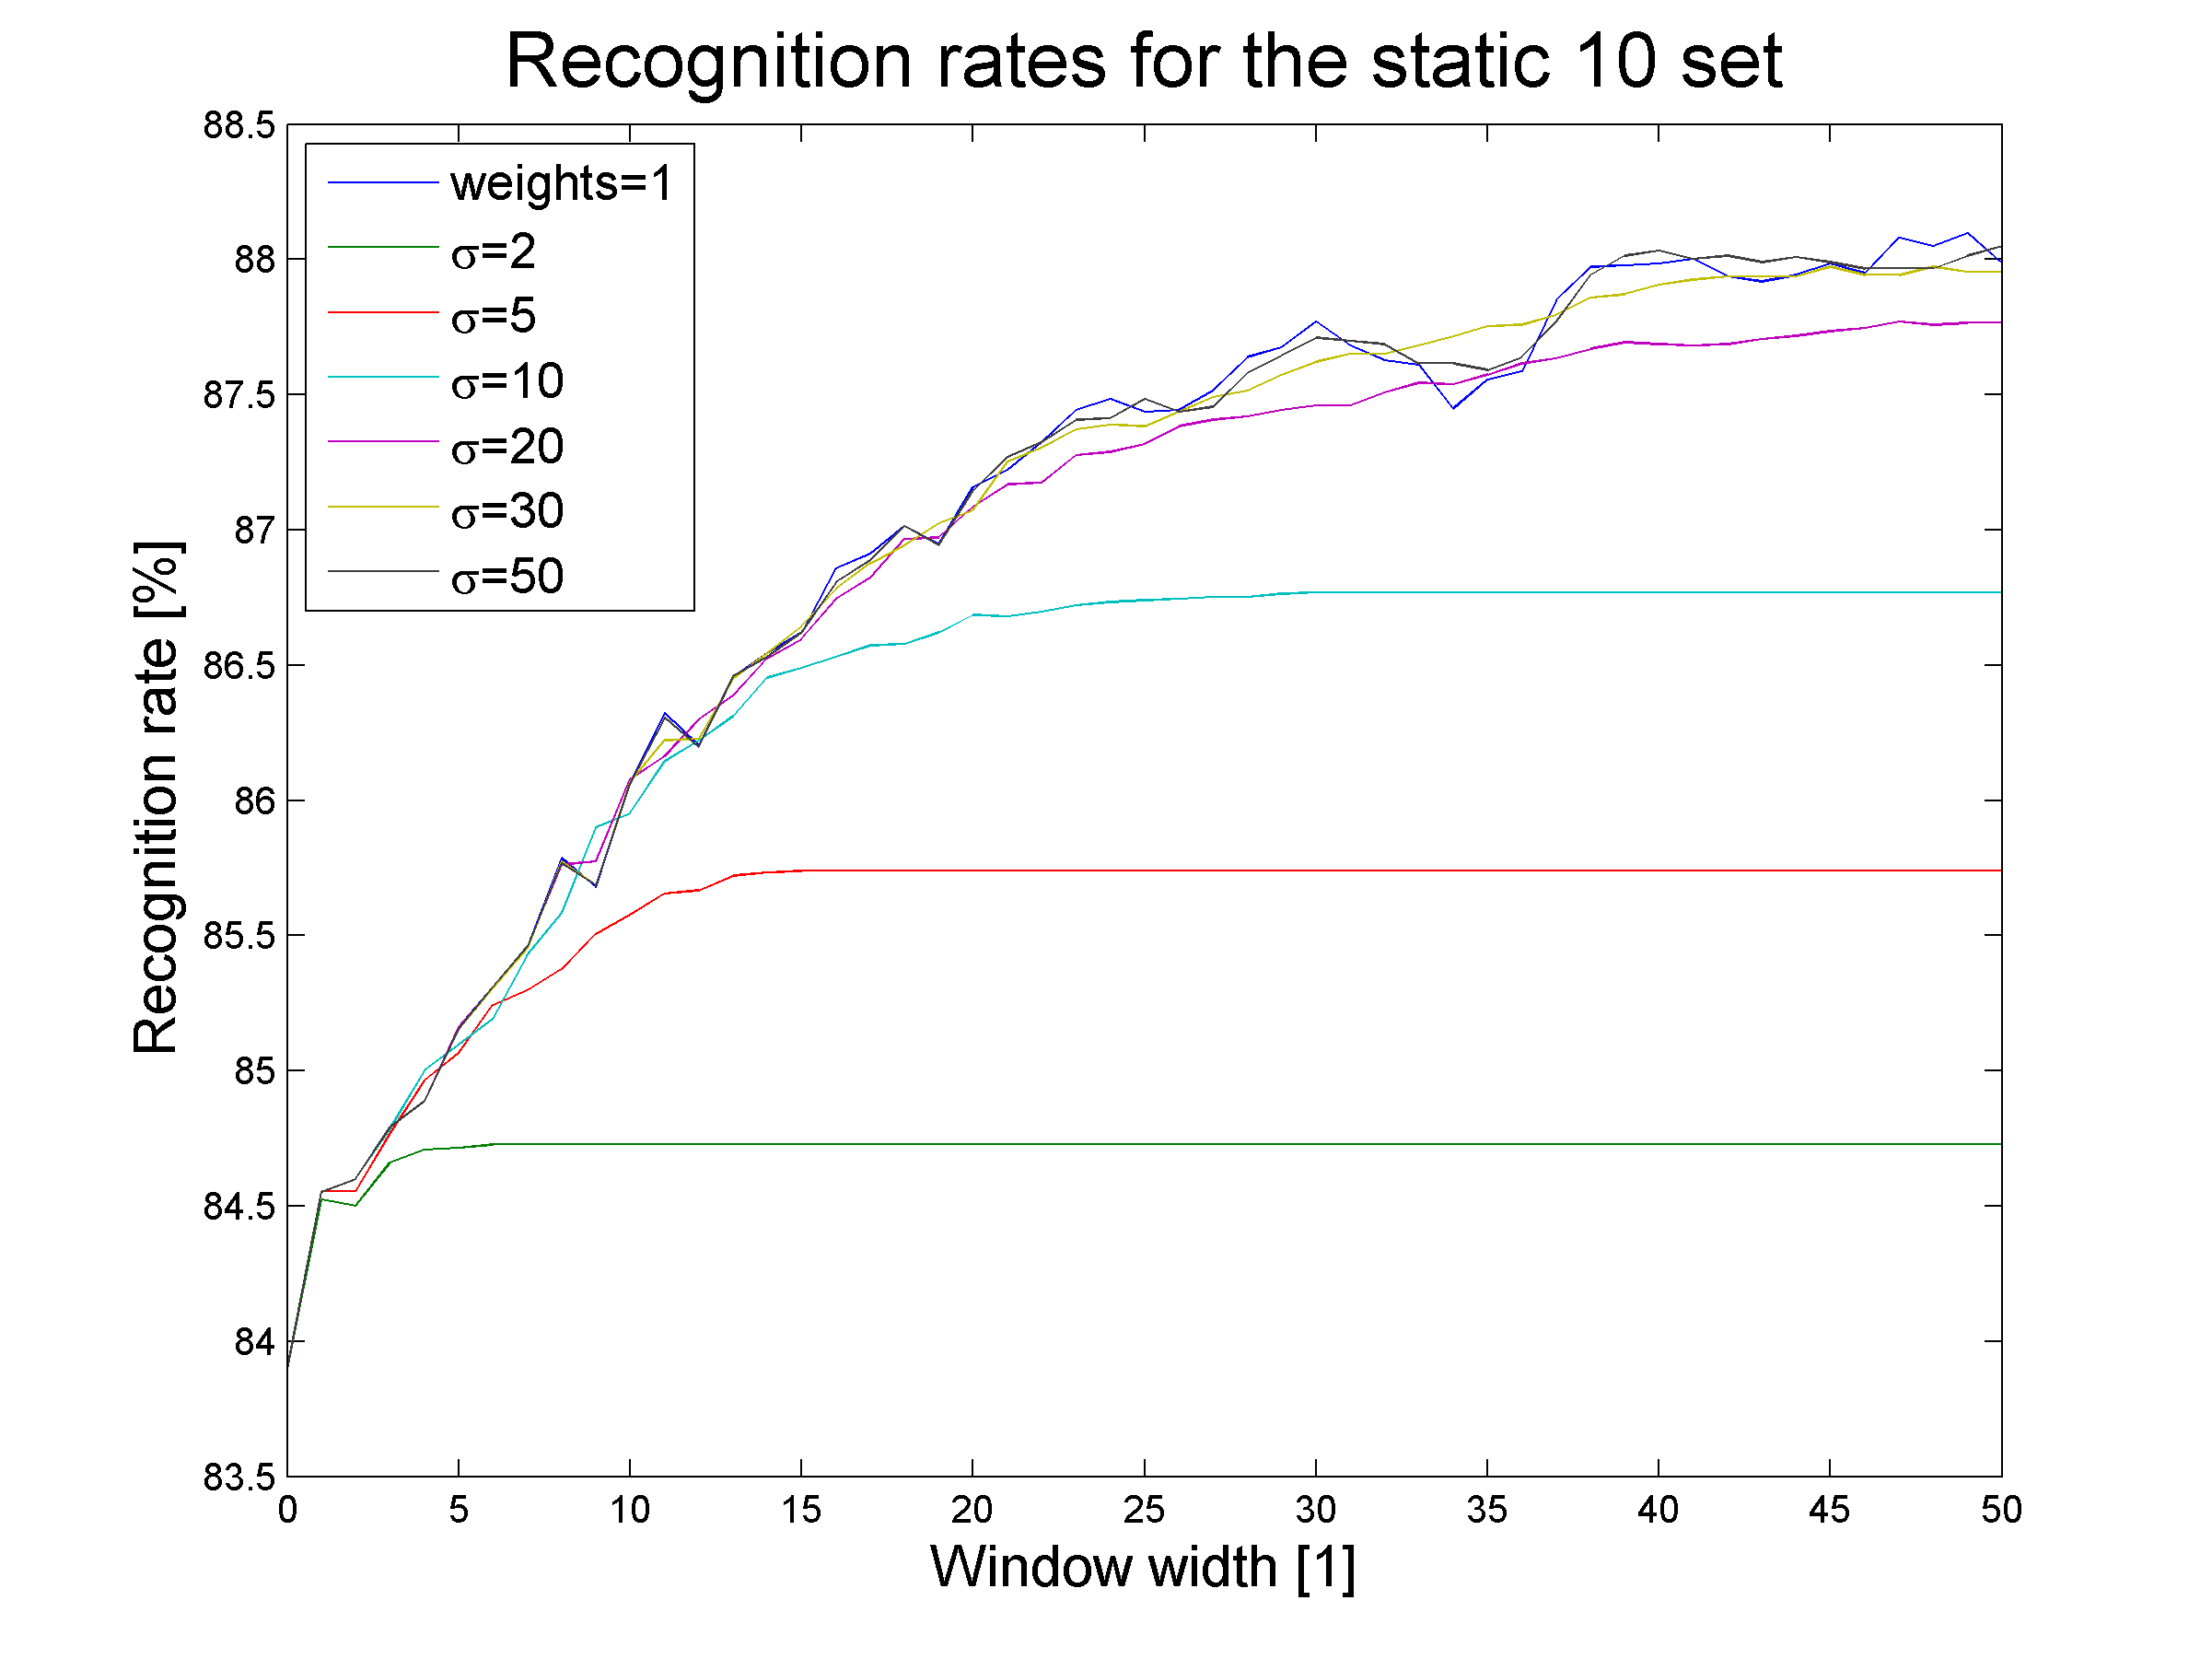
\includegraphics[width=0.7\textwidth]{figures/gaussSum10.png}
 
 \caption{Evaluation of weights for postprocessing distributed accordingly to normal distribution}
 \label{staticgauss}
\end{figure}

For this task, the weights can be taken from half of the Gaussian distribution with maximal peak reached for the currently achieved result with weights slowly decreasing for measurements further away in time.
For Gaussian, the mean was assumed to be equal to $0$.
The standard deviation $\sigma$ was the parameter, for which different values were tested.
The results were obtained on the 5 and 10 static gestures.
The achieved results are presented in Fig.~\ref{staticgauss}.
For 5 gestures, small $\sigma$ resulted in the weights equal to $0$ for the wider window size and therefore not using the whole information available in the specified window. 
For greater $\sigma$, it can be observed that the achieved recognition rate is similar.
The $\sigma$ value equal to $10$ resulted in the best recognition for almost all window sizes.
For problem of 10 static gestures recognition problem, greater $\sigma$ values produced results that are comparable to the results achieved with the summation as aggregation function.
The usage of different weights also comes with greater computing cost.
This approach did not allow to increase the recognition rate and can be omitted without effecting the recognition.

From the presented results, the summation is recommended as the aggregation operator by the authors of this thesis.


\section{Finger recognition} 
Finger recognition module is responsible to verify which particular fingers are detected during gesture recognition. The module can be used for additional processing on the user side, for which the information about the visible fingers can often be significant, It can also assist interpretation of data derived from parametrized gestures. The user can also use the module to better fit dataset features to the characteristics of selected gestures.
\subsection{Methods}
For this module the same classification algorithms (kernel functions) were used as those which had the best results in static gesture recognition. As in the case of static gesture recognition libSVM library has been used and RBF kernel has been selected.
\subsection{Evaluation methodology}
In the assumptions for static gesture recognitions it was mentioned that the process must be independent of the position, rotation, sizes of hand and fingers. This presumption applies also to finger recognition. However, this assumption is still does not contain one element, from which the recognition process should be independent -- arrangement of hand. Whether forefinger is straight or bent, it is the same class, where only this one finger is taken out.

\subsubsection{Recorded dataset}
Dataset was collected by two different people. Each of them has recorded 32 classes, which reflect all the possible permutations of fingers arrangements. The next step was to select from 32 gestures, those which are the most frequently used by people in everyday life. Those 15 selected gestures are natural for human and do not cause pain. People use them as specific sign like peace sign. From the dataset four data collections were created used in the experiments:
\begin{itemize}
\item dataset A -- 32 gestures recorded by two people -- this dataset consists of 58614 samples,
\item dataset B -- 15 gestures recorded by two people -- 28729 samples,
\item dataset C -- 32 gestures recorded by one person -- 36190 samples,
\item dataset D -- 15 gestures recorded by one person -- 18611 samples.
\end{itemize}

\subsection{Features}
As mentioned in the previous section it is important that the fingers recognition process is independent of things like position of hand or size of finger. Thus, 6 features were selected, which are independent of following parameters. 

\begin{figure}[htb]
\centering
 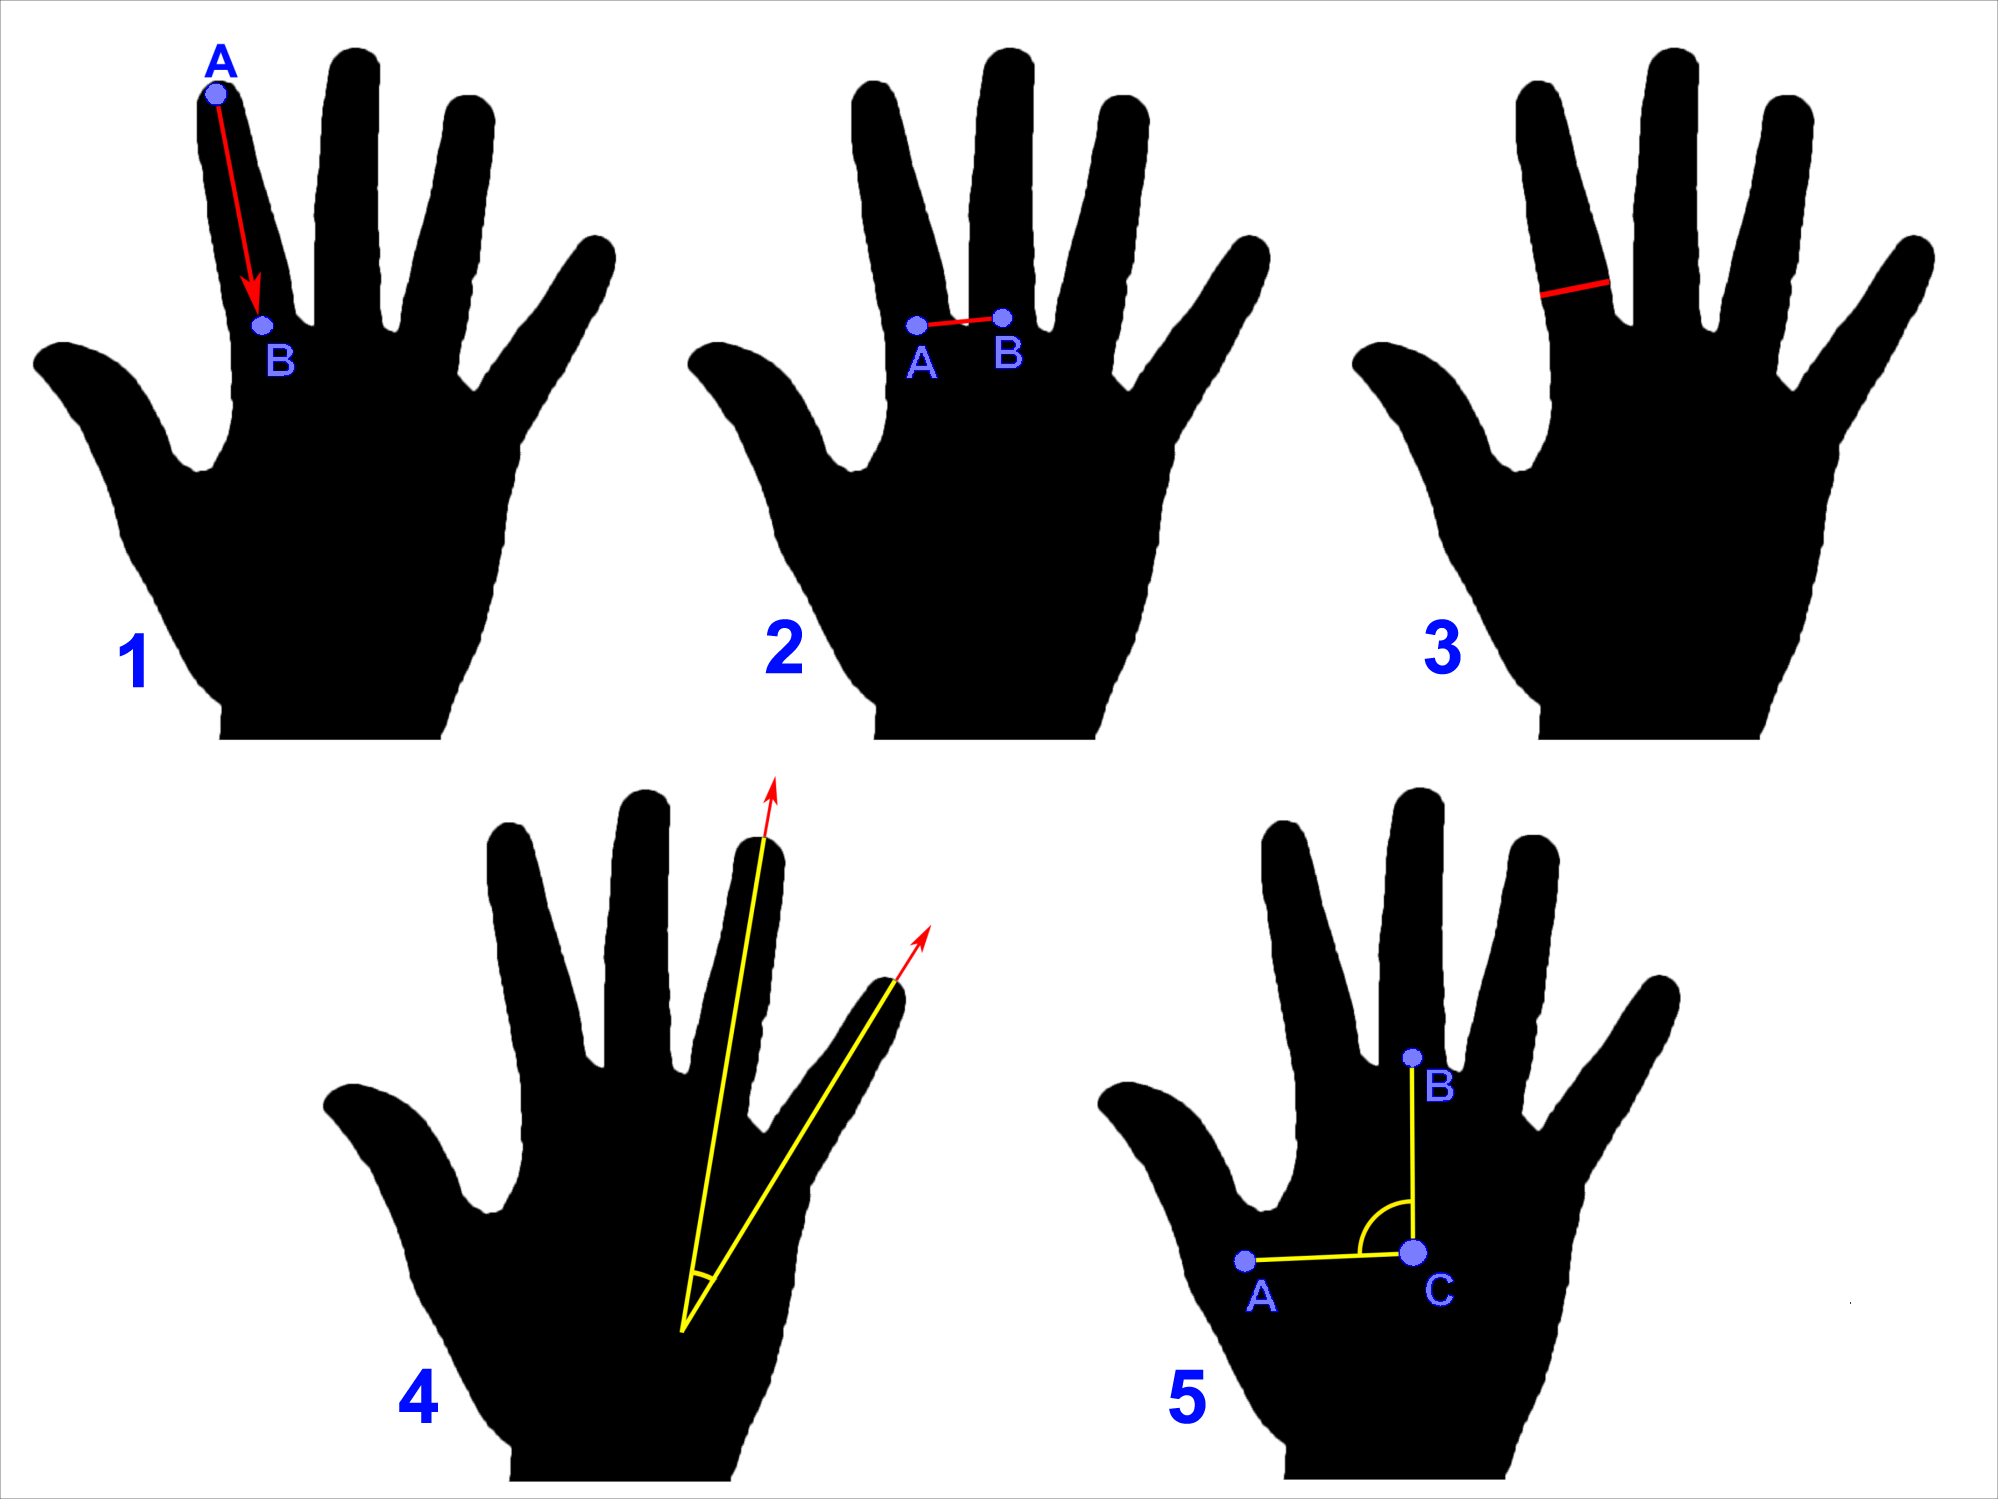
\includegraphics[width=0.75\columnwidth]{figures/fingDiffFeatures.png}
 \caption{Features used for finger recognition}
 \label{fingfifffeatures}
\end{figure}

\begin{enumerate}
\item Finger count. 
\item Distance between two nearest base points of a finger (example of base point has been marked in Fig.~\ref{fingfifffeatures}.1 as point B).
To appoint a finger base point has to be reversed normalized direction vector multiplied by the length of a finger. Subsequent as the beginning of the vector thus formed is set finger tip position. The end of the vector indicates the finger base point (Fig.~\ref{fingfifffeatures}.1). An example of distance between two nearest base points of a finger is showed in Fig.~\ref{fingfifffeatures}.2.
\item Ratio of a finger's thickness to the maximal finger's thickness. 
Leap Motion controller can return information about the thickness of the fingers (Fig.~\ref{fingfifffeatures}.3). There are known relationships between the thicknesses of the fingers, for example that the thumb is the thickest finger. Just like in the previous feature ratio was used in order to become independent of size of finger.
\item Angles between two nearest fingers.
In Fig.~\ref{fingfifffeatures}.4  this feature has been shown. It is obtained by calculating the angle between the direction vectors of two adjacent fingers.
\item Angles between a given finger and the first finger relative to palm position. 
To calculate this angle three positions are needed : two finger tip positions and a palm position. The next step is to determine the line segments between palm position and finger tip positions. The searched angle is between two designated segments. This angle is shown in Fig.~\ref{fingfifffeatures}.5.
\end{enumerate}

During testing a new feature was created based on the feature 2:\newline
2b. ratio of distance between two nearest base points of a finger to the minimal (non-zero) distance between two nearest base points
This feature is very similar to the previous one. The difference is that in this case ratio of distances is used instead of the actual values. Thanks to this, this feature is independent of the size of hand.

\section{Experiments}
Tests were performed using cross validation and test set. In the case of the test set ratio of training set to testing set was 2:1.

For the tests created several combinations of previously described features:
\begin{itemize}
\item 1,2,4
\item 1,3,5
\item 1,3,4,5
\item 1,2,3,4,5
\end{itemize}

All sets of features have been tested for all four datasets. The recognition rate can be seen in Table~\ref{findiff}. It can be concluded that the best match is when the all features are used. However, feature 2 is not independent of the size of the hand. Therefore, a new feature has been designed using the ratio of two values obtained from the original feature. Then the test was performed for a set of: 1, 2b, 3, 4, 5 for all data sets. The result for this test is in the last line of the Table~\ref{findiff}. Interestingly, despite the fact that the modified feature is independent of the size of hand, attribute 2b had an inferior result than the original feature, which operates on the actual value of the distance between fingers. 

\begin{table}[htp!]
\begin{center}
	\label{findiff}
	\caption{Results obtained by experimental feature sets for different data collections}
    \begin{tabular}{|p{1.3cm}|p{1.3cm}|p{1.3cm}|p{1.3cm}|p{1.3cm}|p{1.3cm}|p{1.3cm}|p{1.3cm}|p{1.3cm}|}
    \hline
    features & dataset A, CV[\%] & dataset A, test set[\%] & dataset B, CV[\%] & dataset B, test set[\%] & dataset C, CV[\%]& dataset C, test set[\%]  & dataset D, CV[\%] & dataset D, test set[\%]  \\ \hline
    1,2,4	& 75.4\% & 74.9\% & 87.3\%  & 86.9\% & 78.4\% & 77.9\% & 90.6\% & 90.3\% \\ \hline
    1,3,5     	& 76.3\% & 75.4\% & 87.5\%  & 87.1\% & 79.6\% & 78.9\% & 91.5\% & 91.2\% \\ \hline
    1,3,4,5    	& 78.1\% & 75.4\% & 87.5\%  & 87.1\% & 79.6\% & 78.9\% & 91.5\% & 91.2\% \\ \hline
    1,2,3,4,5   & 83.2\% & 81.5\% & 90.3\%  & 89.8\% & 85.8\% & 85.1\% & 93.0\% & 92.8\% \\ \hline
    1,2b,3,4,5	& 76.6\% & 75.8\% & 87.6\%  & 87.3\% & 79.8\% & 79.2\% & 91.6\% & 91.2\% \\ \hline
    \end{tabular}
    \end{center}
\end{table}

It is worth to mention that it seemed that the feature 4 (angles between two nearest fingers) will have a substantial contribution to finger recognition. However, the results showed that this feature has impact only on the largest amount of data, while in other cases brought nothing.

Distinguishing coefficient of particular classes for a set of features: 1, 2, 3, 4, 5 for 15 classes recorded by two people is shown in Fig.~\ref{classRateFD}.
The graph indicates that classes with the worst recognition rates are:
\begin{itemize}
\item the clenched fist (no fingers), and
\item the hand with stretched out index finger.
\end{itemize}
The rest of the gesture recognition has a level of approximately 90\% and above. Based on these tests can be deduced that the fewer fingers to differentiate, the worse the outcome is. This is due to the characteristics of the feature sets, because the vast majority of the features is based on dependency between two fingers. So when the number of fingers is low, module receives less information, which it uses to fingers recognition.

\begin{figure}[htb]
\centering
 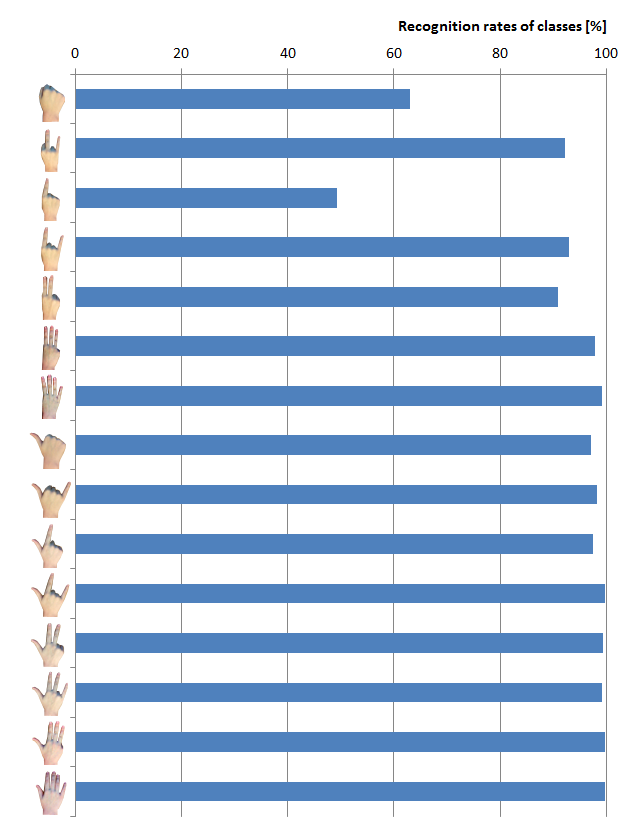
\includegraphics[width=0.75\columnwidth]{figures/classRateFD.png}
 \caption{Recognition rates of 15 classes for finger recognition using dataset B}
 \label{classRateFD}
\end{figure}

In the second round of tests was verified how preprocessing will affect the finger recognition process. For the best set of features from the previous test was performed a new test with preprocessing for all datasets. For tests the preprocessing width of 4 was chosen.

\begin{table}[htp!]
\begin{center}
	\label{findiffpre}
	\caption{Comparison of the recognition rate achieved with and without preprocessing with feature set 1,2,3,4,5}
    \begin{tabular}{|p{1.3cm}|p{1.3cm}|p{1.3cm}|p{1.3cm}|p{1.3cm}|p{1.3cm}|p{1.3cm}|p{1.3cm}|p{1.3cm}|}
    \hline
    features & dataset A, CV[\%] & dataset A, test set[\%] & dataset B, CV[\%] & dataset B, test set[\%] & dataset C, CV[\%]& dataset C, test set[\%]  & dataset D, CV[\%] & dataset D, test set[\%]  \\ \hline
    with preprocessing          & 83.3\% & 82.8\%  & 90.5\% & 90.0\% & 86.5\% & 86.0\% & 93.3 \% & 93.0\% \\ \hline
    without preprocessing   	& 83.2\% & 81.5\% & 90.3\%  & 89.8\% & 85.8\% & 85.1\% & 93.0\% & 92.8\% \\ \hline
    \end{tabular}
    \end{center}
\end{table}

Table~\ref{findiffpre} presents the test results for a set of features: 1, 2, 3, 4, 5 with and without preprocessing. It can be concluded that the use of preprocessing in finger recognition slightly improved the recognition rate. This may be due to selected window width, which makes that while preprocessing is working on one specific frame, it takes into account nine contiguous frames. In this setting small irregularities in the data are corrected. If the window would be bigger, anomalies lasting several tens of frames would also be detected. In this situation, new problems would arise, for example, transitions between classes would be much later detected and thus there would be a lot of long lasting incorrect recognitions.




